\documentclass[sigplan,screen,review]{acmart}

\copyrightyear{2023}
\acmYear{2023}
% \acmDOI{XXXXXXX.XXXXXXX}

%% These commands are for a PROCEEDINGS abstract or paper.
\acmConference[Preprint]{TBD}{Mrach,
  2023}{Charlottesville, VA}

\acmBooktitle{Technical Report University of Virginia, Biocomplexity institute and Initiative, March, 2023, CHarlottesville, VA, U.S.A.} 

\acmPrice{15.00}
\acmISBN{978-1-4503-XXXX-X/18/06}

%%%%%%%%%%%%%%%%%%%%%%%%%%%%%%%%%%%%%%%%%%%%%%%%
%
% REMOVE ACM PAPER INFO
%
\setcopyright{none}
\settopmatter{printacmref=false} % Removes citation information below abstract
\renewcommand\footnotetextcopyrightpermission[1]{} % removes footnote with conference information in first column
\pagestyle{plain}
%%%%%%%%%%%%%%%%%%%%%%%%%%%%%%%%%%%%%%%%%%%%%%%%


\begin{document}

\title{OSMI Benchmark}


\author{Nate Kimbal}
\affiliation{%
  \institution{University of Virginia}
  \streetaddress{Biocomplexity Institute\\
                Town Center Four\\
                994 Research Park Boulevard}
  \city{Charlottesville}
  \state{VA}
  \postcode{22911}
  \country{USA}
}

\author{Wes Brewer}
\affiliation{%
  \institution{Oak Ridge National Laboratory}
  \streetaddress{1 Bethel Valley Road}
  \city{Oak Ridge}
  \state{TN}
  \postcode{37830}
  \country{Iceland}}
\email{larst@affiliation.org}

\author{Gregor von Laszewski}
\email{laszewski@gmail.com}
\orcid{0000-0001-9558-179X}
\affiliation{%
  \institution{University of Virginia}
  \streetaddress{Biocomplexity Institute\\
                Town Center Four\\
                994 Research Park Boulevard}
  \city{Charlottesville}
  \state{VA}
  \postcode{22911}
  \country{USA}
}

\author{Geoffrey C. Fox}
\affiliation{%
  \institution{University of Virginia}
  \streetaddress{Biocomplexity Institute\\
                Town Center Four\\
                994 Research Park Boulevard}
  \city{Charlottesville}
  \state{VA}
  \postcode{22911}
  \country{USA}
}


% \renewcommand{\shortauthors}{Trovato and Tobin, et al.}

%%
%% The abstract is a short summary of the work to be presented in the
%% article.
\begin{abstract}
  TBD

  TODO: fix CCSXML, ccsdec
\end{abstract}

\begin{CCSXML}
<ccs2012>
   <concept>
       <concept_id>10002951.10003227.10003241.10003244</concept_id>
       <concept_desc>Information systems~Data analytics</concept_desc>
       <concept_significance>500</concept_significance>
       </concept>
   <concept>
       <concept_id>10010520.10010521.10010537.10003100</concept_id>
       <concept_desc>Computer systems organization~Cloud computing</concept_desc>
       <concept_significance>500</concept_significance>
       </concept>
   <concept>
       <concept_id>10011007.10011006.10011072</concept_id>
       <concept_desc>Software and its engineering~Software libraries and repositories</concept_desc>
       <concept_significance>500</concept_significance>
       </concept>
 </ccs2012>
\end{CCSXML}

\ccsdesc[500]{Information systems~Data analytics}
\ccsdesc[500]{Computer systems organization~Cloud computing}
\ccsdesc[500]{Software and its engineering~Software libraries and repositories}


% up to 5 keywords
\keywords{benchmark, deep learning, mlcommons}

\received{March 2023}
%\received[revised]{12 March 2009}
%\received[accepted]{5 June 2009}

 %%%%%%%%%%%%%%%%%%%%%%%%%%%%%%%%%%%%%%%%%%%%%%%%
% next line can be removed if submitted to acm
\settopmatter{printfolios=true}
%%%%%%%%%%%%%%%%%%%%%%%%%%%%%%%%%%%%%%%%%%%%%%%%

\maketitle

\section{Introduction}

TBD


\section{OSMI}

what is the application


\section{Benchmark}

\subsection{Hardware}

\paragraph{WSL.} - Nate

\paragraph{Ubuntu.} - Gregor

\paragraph{Rivanna.} - Nate

It contains a variety of GPU-enabled nodes. This includes
GPUs of type RTX2080, V100, P100, K80,   A100 (40GB), and A100 (80GB). The file system is centralized and accessible via NFS. 

\paragraph{Filesystem Comparision}

We provide here the comparison of the file system that is motivated by observations made in \cite{???}.


TODO: include table



\subsection{Results}


\section{Examples for Tables and Images}

Table~\ref{tab:freq} shows ...

\begin{table}
  \caption{Frequency of Special Characters}
  \label{tab:freq}
  \begin{tabular}{ccl}
    \toprule
    Non-English or Math&Frequency&Comments\\
    \midrule
    \O & 1 in 1,000& For Swedish names\\
    $\pi$ & 1 in 5& Common in math\\
    \$ & 4 in 5 & Used in business\\
    $\Psi^2_1$ & 1 in 40,000& Unexplained usage\\
  \bottomrule
\end{tabular}
\end{table}


\begin{figure}[h]
  \centering
  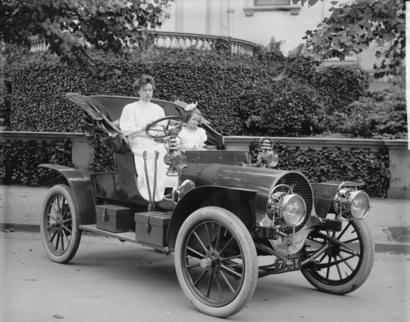
\includegraphics[width=1.0\linewidth]{images/sample-franklin.png}
  \caption{1907 Franklin Model D roadster. Photograph by Harris \&
    Ewing, Inc. [Public domain], via Wikimedia
    Commons. (\url{https://goo.gl/VLCRBB}).}
    \label{fig:womman-girl}
  \Description{A woman and a girl in white dresses sit in an open car. Use PDF images and also create 300/600dpi png images. for online its also good to do svg. So if you can create all versions. photos are only png.}
\end{figure}

Figure \ref{fig:womman-girl} shows a
a woman and a girl in white dresses sit in an open car. Use PDF images and also create 300/600dpi png images. for online its also good to do svg. So if you can create all versions. photos are only png.

\section{Examples Citation}

Example \cite{cloudmesh-hybrid-workflow}

%%%%%%%%%%%%%%%%%%%%%%%%%%%%%%%%%%%%%%%%%%%%%%%%%%%%%%%%%%%%%

\begin{acks}

We like to thank ...

TBD. DOE, NSF, NIST
To Robert, for the bagels and explaining CMYK and color spaces.
\end{acks}

%%%%%%%%%%%%%%%%%%%%%%%%%%%%%%%%%%%%%%%%%%%%%%%%%%%%%%%%%%%%%

\bibliographystyle{ACM-Reference-Format}
\bibliography{paper}

%%%%%%%%%%%%%%%%%%%%%%%%%%%%%%%%%%%%%%%%%%%%%%%%%%%%%%%%%%%%%
\appendix
%%%%%%%%%%%%%%%%%%%%%%%%%%%%%%%%%%%%%%%%%%%%%%%%%%%%%%%%%%%%%

\section{Online Resources}

\begin{description}

\item{Code}
\item{Cloudmesh-common}
\item{Cloudmesh-StopWatch}
\item{Mlcommons}

\end{description}

\end{document}

\endinput
%%
%% End of file `sample-sigplan.tex'.
